\documentclass{article}
\usepackage{arxiv}

\usepackage[utf8]{inputenc}
\usepackage[english, russian]{babel}
\usepackage[T1]{fontenc}
\usepackage{url}
\usepackage{booktabs}
\usepackage{amsfonts}
\usepackage{nicefrac}
\usepackage{microtype}
\usepackage{lipsum}
\usepackage{graphicx}
\usepackage{natbib}
\usepackage{doi}



\title{Декодирования сигналов головного мозга в аудиоданные}

\author{ Набиев Мухаммадшариф \\
        Кафедра интеллектуальных систем\\
	МФТИ\\
	\texttt{nabiev.mf@phystech} \\
	\And
	Северилов Павел \\
	Кафедра интеллектульных систем\\
	МФТИ\\
	\texttt{pseverilov@gmail.com} \\
	%% \AND
	%% Coauthor \\
	%% Affiliation \\
	%% Address \\
	%% \texttt{email} \\
	%% \And
	%% Coauthor \\
	%% Affiliation \\
	%% Address \\
	%% \texttt{email} \\
	%% \And
	%% Coauthor \\
	%% Affiliation \\
	%% Address \\
	%% \texttt{email} \\
}
\date{}

\renewcommand{\shorttitle}{\textit{arXiv} Template}

%%% Add PDF metadata to help others organize their library
%%% Once the PDF is generated, you can check the metadata with
%%% $ pdfinfo template.pdf
\hypersetup{
pdftitle={Декодирования сигналов головного мозга в аудиоданные},
pdfsubject={q-bio.NC, q-bio.QM},
pdfauthor={Набиев Мухаммадшариф, Северилов Павел},
pdfkeywords={First keyword, Second keyword, More},
}

\begin{document}
\maketitle

\begin{abstract}
  В данной работе исследуется проблема декодирования сигналов головного мозга в аудиосигналы с использованием физически-информированных методов получения эмбеддингов сигналов. Предлагается решить задачу классификации стимулов по соответствующим сегментам аудиоданных. Под стимулом понимается аудиосигнал, который вызвал активность мозга, соответствующая ЭЭГ-сигналу. Данные для задачи представляют собой 668 пар вида ЭЭГ-стимул общей продолжительностью стимулов 9431 минута. В качестве метрики для выбора оптимальной модели используется F1-мера. В данной работе предлагается исследовать передовые методы машинного обучения, которые учитывают физические принципы, с целью улучшения качества обработки аудиосигналов и повышения точности их декодирования. Полученные результаты имеют важное значение для развития интерфейсов мозг-компьютер и понимания принципов обработки аудиосигналов человеческим мозгом.

\end{abstract}


\keywords{auditory EEG decoding \and natural speech processing \and EEG}

\section{Введение} 
    \par 
    Слух, одно из наиболее важных человеческих чувств, играет решающую роль в нашем повседневном взаимодействии с окружающим миром. Однако многие люди со всего мира сталкиваются с проблемами слуха, которые могут серьезно ограничить их способность воспринимать звуки окружающей среды. В свете этих проблем возникает интерес к исследованию взаимосвязи между звуком и мозговыми сигналами. В данной области выделена задача декодирования мозговых сигналов в аудиоданные. 
    \par 
    Задачу декодирования можно поставить двумя способами: классификация и регрессия. В данной работе мы сконцентрируемся на задаче классификации. Требуется решить задачу классификации в парадигме match-mismatch, когда на вход подается ЭЭГ сигнал и 5 стимулов, из которых только один соответствует сигналу. Под стимулом подразумевается сегмент аудио, который стимулировал сигнал в мозгу субъекта. 
    \par 
    Существует базовое решение этой задачи, использующее расширенную сверточную сеть~\citep{Accou2021ModelingTR}. Эта сверточная сеть используется в качестве энкодера ЭЭГ и стимула.
    \par 
    Известна модификация базового решения с использованием Multi-Head Attentionи и GRU~\citep{multihead-gru}. Дополнительно авторы генерируют также и спектрограмму для получения дополнительных признаков, как, например, частота. Также в отличие от базового решения стимулы и спектрограммы проходят через GRU, а уже потом подаются на вход в энкодер. 
    \par 
    В постановке классификации из наиболее успешных были работы, которые учитывали особенности речи, такие как частоту и пол. Работа~\citep{Thornton2023RelatingER} показала высокую чувствительность ЭЭГ-сигнала от основной частоты. Значительные улучшения качеств были достигнуты за счет ансамблирования моделей. Хоть и выделение основной частоты повысило качество в целом, было выяснено, что такой подход сильно зависит от пола говорящего~\citep{Puffay2022RelatingTF}. На качество классификации также влияет частота дискретизации, как это показано в работе~\citep{Thornton2024DetectingGR}. В этой постановке особенно хорошо показали себя модели, которые использовали физические информированные энкодеры для стимула, а также их спектрограммы~\citep{Wang2024SelfsupervisedSR}.
    \par
    Решению задачи декодирования в постановке регрессии посвящена статья~\cite{piao2023happyquokka}. Авторами была предложена модель Pre-LLN FFT, основанная на модели Feed-Forward Transformer(FFT) network из \citep{ren2019fastspeech}. За счет модификации FFT и добавления global conditioner~\citep{vandenoord16_ssw} и нормализации пред-слоя~\citep{xiong2020layer}, авторы добились улучшения коэффициента корелляции Пирсона по сравнению с базовым решением использовавшим Very Large Augmented Auditory Inference(VLAAI)~\citep{vlaai}. 

    Для решения задачи классификации предлагается использовать физически-информированные энкодры для стимулов, и их спектрограммы, а также воспользоваться трансформером для захвата деталей активности мозга по ЭЭГ-сигналу.

\section{Постановка задачи}    
    Каждый объект представляет собой кортеж $(\mathbf{X}^i, \mathbf{s}_1^i, \dots, \mathbf{s}_K^i)$, где $\mathbf{X}^i \in \mathbb{R}^{64 \times T}$~--- ЭЭГ-сигнал, $\mathbf{s}_1^i, \dots, \mathbf{s}_K^i \in \mathbb{R}^{1 \times T}$--- стимулы, а $K$~--- количество стимулов. Под стимулом понимается огибающая аудиосегмента длительностью $T$(Рис.~\ref{envelope}). Меткой данного объекта будет являться вектор $\mathbf{y}^i \in \mathbb{R}^K$. Метка имеет только одну координату равную единице, которая соответствует стимулу, спровоцировавшему ЭЭГ-сигнал. Требуется по имеющимся $\mathbf{X}^i, \mathbf{s}_1^i, \dots, \mathbf{s}_K^i$ получить распределение вероятностей стимулов $\mathbf{p}^i = [p_1^i, \dots , p_K^i]^T$. Пусть модель представляет собой следующее отображение $\mathbf{F} : \mathbb{R}^{64 \times T} \times \left( \mathbb{R}^{1\times T} \right)^K \rightarrow \mathbb{R}^5$. Задача сводится к минимизации Cross-Entropy Loss:
    $$CE = - \frac{1}{N}\sum_{i=1}^N\sum_{k=1}^K y_k^i \log \left( \left[ \mathbf{F}(\mathbf{X}^i, \mathbf{S}^i) \right]_k \right),$$
    где $\mathbf{S}^i = (\mathbf{s}^i_1, \dots, \mathbf{s}^i_K)$. То есть решается задача мультиклассовой классификации.

\subsection{Описание методов}
    Схема модели представлена на Рис.~\ref{model}
    \begin{figure}[h]
        \centering
        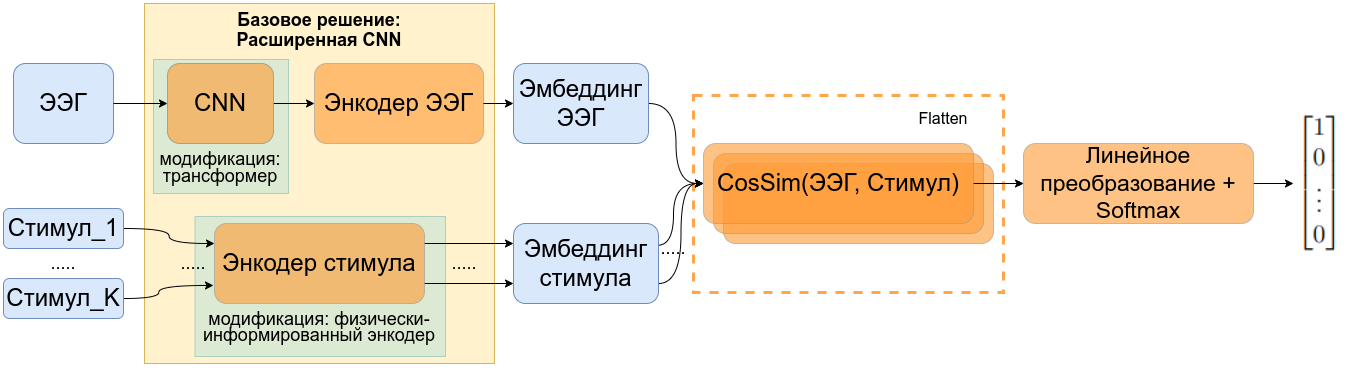
\includegraphics[scale=0.35]{model_architecture.png}
        \caption{Предложенная модель. Базовое решение представляет собой расширенную CNN в качестве энкодера ЭЭГ и стимула с общими весами. Также в базовом решении размерность ЭЭГ уменьшают с помощью одномерной свертки. Предлагается использовать трансформер для ЭЭГ, а для стимула поменять CNN на физически-информированный энкодер.}
        \label{model}
    \end{figure}

    \subsection{Базовое решение}
    В базовом решении используется расширенная сверточная сеть, в качестве энкодера ЭЭГ и стимулов с общими весами. Отметим, что все свертки одномерные. В начале сверточный слой с 8 фильтрами  и ядром $1 \times 1$ объединяет информацию по всем 64 каналам и уменьшает размерность. Преобразованная матрица $\mathbf{X}_1 = \mathrm{Conv}(\mathbf{X}, K_1)$, где $K_1$~--- ядро слоя, а $\mathbf{X}$~--- ЭЭГ-сигнал, имеет размерность $8 \times T$. Энкодер ЭЭГ в базовом решении представляет собой $n$ блоков расширенной сверточной сети. Блоки идентичные и каждый из них имеет 16 фильтров с ядрами $3 \times 3$. Ядра на каждом слое в пределах одного блока будут разными. Например, для слоя $L_m$ ядро $K_2^m$ будет иметь коэффициент расширения равному $3^{m-1}$. Описанный энкодер ЭЭГ дает скрытое представление матрицы $\mathbf{X}_1$, обозначим его $\mathbf{E}$, в латентном пространстве $\mathbb{R}^{16 \times T'}$. Аналогично получаем скрытое представление стимулов $\mathbf{P}_1, \dots, \mathbf{P}_K$ в том же латентном пространстве, за исключением того, что стимулы сразу проходят через $n$  блоков энкодера.
    
    Получив скрытые представления высчитывается их близость в пространстве, как произведение матриц $\mathbf{C}_k = \mathrm{CosSim}(\mathbf{E}, \mathbf{P}_k) = \mathbf{E} \mathbf{P}_k^T$. После линейного преобразования и функции \operatorname{SoftMax} получаем итоговое распределение вероятностей.

    \subsection{Улучшения}
    Пространственное преобразование ЭЭГ -> трансформер.

    Энкодер стимула -> физически-информированный энкодер.

\section{Вычислительный эксперимент}
\subsection{Данные}
    Эксперимент будет проверяться на данных~\citep{K3VSND_2023}. Они представляют собой выборку из 85 человек. Все участники прослушали 6, 7, 8 или 10 стимулов, каждая из которых имеет примерную продолжительность 15 мин. После прослушивания участников спрашивали про содержания аудиофрагмента. Это было с целью мотивировать участников обращать внимания во время прослушивания.

    Стимулы были разделены на следующие категории:

    \begin{itemize}
        \item Референсные аудиокниги
        \item Аудиокниги для детей и взрослых. Если длина превышала 15 мин, то аудиокнига делилась на части
        \item Аудиокниги с шумом
        \item Подкасты про ответы на научные вопросы
        \item Подкасты с видео
    \end{itemize}

    Также отметим, согласно авторам, что частота дискретизации ЭЭГ и стимулов была занижена до 64 Гц. А обработанные стимулы представляют собой огибающую кривую сигнала аудиофрагмента.
    
    \begin{figure}[h]
	\centering
	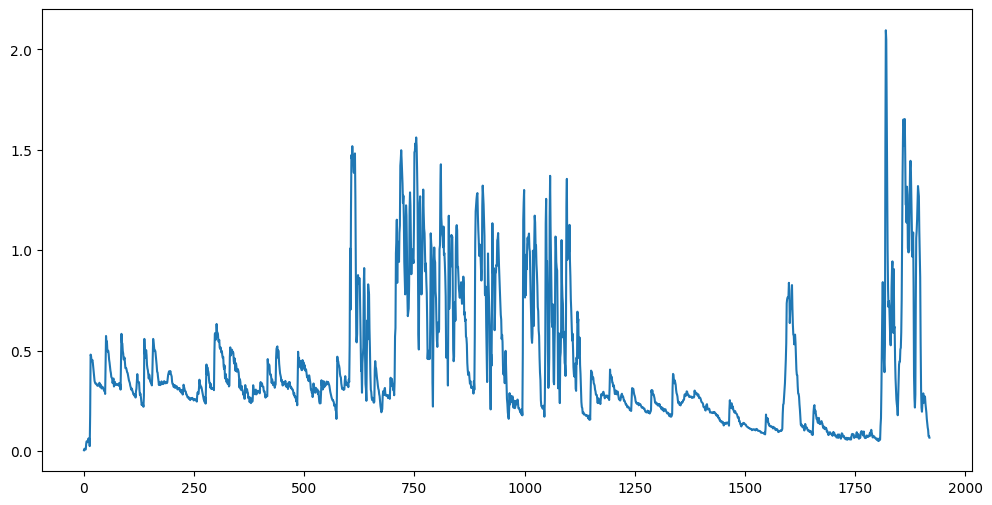
\includegraphics[width=0.7\textwidth]{presented_stimuli.png}
	\caption{Пример огибающей сигнала}
	\label{envelope}
    \end{figure}

    В данных имеется дисбаланс полов, конкретно 74 женщин и 11 мужчин. Так как особенности речи у мужчин и женщин сильно отличаются, для предотвращения переобучения было принято решение отобрать случайно 11 женщин. Для проведения эксперимента данные были разбиты на тренировочную, валидационную и тестовую части в соотношении $80\% : 10\%  : 10\%$. 

    % \subsection{Предобработка данных}
    

    \subsection{Описание эксперимента}    
    Для эксперимента ширина окна была взята равной 5 секунд. Количество стимулов $K=5$, то есть один истинный стимул и четыре ложных. Эксперимент проводился на $10$ эпохах, а один батч представляет собой 16 объектов. В качестве метрики взята точность. 
    
    Для каждого $i$-го объекта/кортежа из выборки у нас может быть только один истинный стимул, следовательно, введем функцию $g : \mathbb{R}^5 \times \mathbb{R}^5 \rightarrow \{0, 1\}$, как 
    $$
        g\left( \mathbf{F}\left( \mathbf{X}^i, \mathbf{S}^i\right), \mathbf{y}^i \right) = \mathbb{I} \left[ \mathbf{y}^i = \mathbf{F}\left( \mathbf{X}^i, \mathbf{S}^i\right) \right].
    $$
    Тогда точность высчитывается, как 
    $$
        Accuracy = \frac{1}{N} \sum_{i=1}^N g\left( \mathbf{F}\left( \mathbf{X}^i, \mathbf{S}^i\right), \mathbf{y}^i \right)
    $$
    % Введем функцию $g : \mathbb{R}^5 \rightarrow \mathbb{R}^5$, которая принимает на вход распределение вероятностей и выдает вектор из нулей и единицы, то есть $\left[ g(\mathbf{p}) \right]_k = \left[ \mathbb{I} \left[p_k = \max_{j\in \{1, \dots, K\}} p_j \right] \right]_k$. Так как классификация, то посчитаем среднее от угаданных меток, более конкретно

        % $$TP_{avg} + TN_{avg} = \frac{1}{K} \sum_{k=1}^K \mathbb{I} \left[ y_k = \left[ g(\mathbf{p}) \right]_k \right]$$

    
 %    Измерения на маленькой части данных. Результаты приведены на графике~\ref{res} 
 %    \begin{figure}[h]
	% \centering
	% 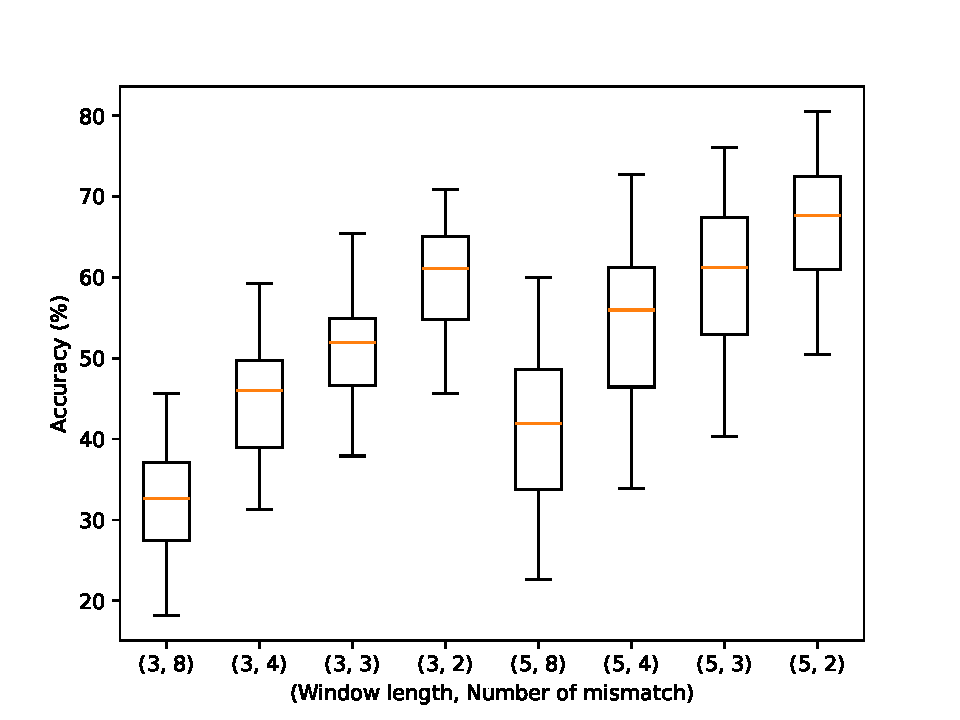
\includegraphics[width=0.7\textwidth]{boxplot_dilated_conv.pdf}
	% \caption{Зависимость точности от размера окна и количества ложных стимулов}
	% \label{res}
 %    \end{figure}
    
    
\bibliographystyle{plain}
\bibliography{Nabiev2024SignalToAudio}

\end{document}